\documentclass[journal,12pt,twocolumn]{IEEEtran}

\usepackage{setspace}
\usepackage{gensymb}
\singlespacing
\usepackage[cmex10]{amsmath}
\usepackage{relsize}
\usepackage{amsthm}
\usepackage{newtxtext}
\usepackage{mathrsfs}
\usepackage{txfonts}
\usepackage{stfloats}
\usepackage{bm}
\usepackage{cite}
\usepackage{cases}
\usepackage{subfig}

\usepackage{longtable}
\usepackage{multirow}

\usepackage[inline]{enumitem}   
\makeatletter
% This command ignores the optional argument for itemize and enumerate lists
\newcommand{\inlineitem}[1][]{%
\ifnum\enit@type=\tw@
    {\descriptionlabel{#1}}
  \hspace{\labelsep}%
\else
  \ifnum\enit@type=\z@
       \refstepcounter{\@listctr}\fi
    \quad\@itemlabel\hspace{\labelsep}%
\fi}
\makeatother
\usepackage{mathtools}
\usepackage{steinmetz}
\usepackage{tikz}
\usepackage{circuitikz}
\usepackage{verbatim}
\usepackage{tfrupee}
\usepackage[breaklinks=true]{hyperref}
\usepackage{graphicx}
\usepackage{tkz-euclide}

\usetikzlibrary{calc,math}
\usepackage{listings}
    \usepackage{color}                                            %%
    \usepackage{array}                                            %%
    \usepackage{longtable}                                        %%
    \usepackage{calc}                                             %%
    \usepackage{multirow}                                         %%
    \usepackage{hhline}                                           %%
    \usepackage{ifthen}                                           %%
    \usepackage{lscape}     
\usepackage{multicol}
\usepackage{chngcntr}
\DeclareMathOperator*{\Res}{Res}

\renewcommand\thesection{\arabic{section}}
\renewcommand\thesubsection{\thesection.\arabic{subsection}}
\renewcommand\thesubsubsection{\thesubsection.\arabic{subsubsection}}

\renewcommand\thesectiondis{\arabic{section}}
\renewcommand\thesubsectiondis{\thesectiondis.\arabic{subsection}}
\renewcommand\thesubsubsectiondis{\thesubsectiondis.\arabic{subsubsection}}


\hyphenation{op-tical net-works semi-conduc-tor}
\def\inputGnumericTable{}                                 %%

\lstset{
%language=C,
frame=single, 
breaklines=true,
columns=fullflexible
}
\begin{document}

\newcommand{\BEQA}{\begin{eqnarray}}
\newcommand{\EEQA}{\end{eqnarray}}
\newcommand{\define}{\stackrel{\triangle}{=}}
\bibliographystyle{IEEEtran}
\raggedbottom
\setlength{\parindent}{0pt}
\providecommand{\mbf}{\mathbf}
\providecommand{\pr}[1]{\ensuremath{\Pr\left(#1\right)}}
\providecommand{\qfunc}[1]{\ensuremath{Q\left(#1\right)}}
\providecommand{\sbrak}[1]{\ensuremath{{}\left[#1\right]}}
\providecommand{\lsbrak}[1]{\ensuremath{{}\left[#1\right.}}
\providecommand{\rsbrak}[1]{\ensuremath{{}\left.#1\right]}}
\providecommand{\brak}[1]{\ensuremath{\left(#1\right)}}
\providecommand{\lbrak}[1]{\ensuremath{\left(#1\right.}}
\providecommand{\rbrak}[1]{\ensuremath{\left.#1\right)}}
\providecommand{\cbrak}[1]{\ensuremath{\left\{#1\right\}}}
\providecommand{\lcbrak}[1]{\ensuremath{\left\{#1\right.}}
\providecommand{\rcbrak}[1]{\ensuremath{\left.#1\right\}}}
\theoremstyle{remark}
\newtheorem{rem}{Remark}
\newcommand{\sgn}{\mathop{\mathrm{sgn}}}
\providecommand{\abs}[1]{\vert#1\vert}
\providecommand{\res}[1]{\Res\displaylimits_{#1}} 
\providecommand{\norm}[1]{\lVert#1\rVert}
%\providecommand{\norm}[1]{\lVert#1\rVert}
\providecommand{\mtx}[1]{\mathbf{#1}}
\providecommand{\mean}[1]{E[ #1 ]}
\providecommand{\fourier}{\overset{\mathcal{F}}{ \rightleftharpoons}}
%\providecommand{\hilbert}{\overset{\mathcal{H}}{ \rightleftharpoons}}
\providecommand{\system}{\overset{\mathcal{H}}{ \longleftrightarrow}}
  %\newcommand{\solution}[2]{\textbf{Solution:}{#1}}
\newcommand{\solution}{\noindent \textbf{Solution: }}
\newcommand{\cosec}{\,\text{cosec}\,}
\providecommand{\dec}[2]{\ensuremath{\overset{#1}{\underset{#2}{\gtrless}}}}
\newcommand{\myvec}[1]{\ensuremath{\begin{pmatrix}#1\end{pmatrix}}}
\newcommand{\mydet}[1]{\ensuremath{\begin{vmatrix}#1\end{vmatrix}}}
\numberwithin{equation}{subsection}
\makeatletter
\@addtoreset{figure}{problem}
\makeatother
\let\StandardTheFigure\thefigure
\let\vec\mathbf
\renewcommand{\thefigure}{\theproblem}
\def\putbox#1#2#3{\makebox[0in][l]{\makebox[#1][l]{}\raisebox{\baselineskip}[0in][0in]{\raisebox{#2}[0in][0in]{#3}}}}
     \def\rightbox#1{\makebox[0in][r]{#1}}
     \def\centbox#1{\makebox[0in]{#1}}
     \def\topbox#1{\raisebox{-\baselineskip}[0in][0in]{#1}}
     \def\midbox#1{\raisebox{-0.5\baselineskip}[0in][0in]{#1}}
\vspace{3cm}
\title{Assignment 6}
\author{Gorantla Pranav Sai- CS20BTECH11018}
\maketitle
\newpage
\bigskip
\renewcommand{\thefigure}{\theenumi}
\renewcommand{\thetable}{\theenumi}
Download all python codes from 
\begin{lstlisting}
https://github.com/pranav-159/ai1103_Probability_and_Random_variables/blob/main/Assignment_6/codes/ExperimentalVerification_Assignment6.py
\end{lstlisting}
%
and latex-tikz codes from 
%
\begin{lstlisting}
https://github.com/pranav-159/ai1103_Probability_and_Random_variables/blob/main/Assignment_6/Assignment6.tex
\end{lstlisting}
\section{Problem}
\textbf{GATE 2015 (EE paper-01 new 2), Q.10 (apti. section)}\\
  The probabilities that a student passes in Mathematics, Physics and Chemistry are m,p, and
c respectively. Of these subjects, the student has 75\% chance of passing in at least one, a
50\% chance of passing in at least two and a 40\% chance of passing in exactly two.
Following relations are drawn in m, p, c:
    \begin{enumerate}[label=(\Roman*)]
        \item p + m + c = 27/20
        \item p + m + c = 13/20
        \item (p)$\times$ (m) $\times$ (c) =1/10
    \end{enumerate}
    \begin{enumerate}[label=(\Alph*)]
      \item Only relation I is true
      \item Only relation II is true
      \item Relations II and III are true
      \item Relations I and III are true
    \end{enumerate}
\section{Solution}
Let M,P,C be the events representing student passes in Mathematics,Physics,Chemistry respectively.
\begin{align}
    \pr{M}&=m\\
    \pr{P}&=p\\
    \pr{C}&=c
\end{align}
The given information can be represented as
\begin{align}
    \pr{M+P+C}=75\%=\dfrac{3}{4}\label{atleast_1}\\
    \pr{MP+PC+CA}=50\%=\dfrac{1}{2}\label{atleast_2}\\
    \pr{MP+PC+CA-3MPC}=40\%=\dfrac{2}{5} \label{only_2}
\end{align}
\eqref{atleast_2} and \eqref{only_2} can also be written as
\begin{align}
    \pr{MP}+\pr{PC}+\pr{CM}&\nonumber\\-2\pr{MPC}&=\dfrac{1}{2}\\
    \pr{MP}+\pr{PC}+\pr{CM}&\nonumber\\-3\pr{MPC}&=\dfrac{2}{5}
\end{align}
Subtracting and solving the above two equations we get,
\begin{align}
    \pr{MPC}&=\dfrac{1}{10}\\
    \pr{MP}+\pr{PC}+\pr{CM}&=\dfrac{7}{10}
\end{align}
Using inclusion-exclusion principle, We can express \eqref{atleast_1} as
\begin{align}
\pr{M}+\pr{P}+\pr{C}&\nonumber\\
-[\pr{MP}+\pr{PC}+\pr{CM}]&\nonumber\\
      +\pr{MPC}&=\dfrac{3}{4}\\
    p+m+c-\dfrac{7}{10}+\dfrac{1}{10}&=\dfrac{3}{4}\\
    p+m+c&=\dfrac{27}{10}
\end{align}
There is no constant answer for the product of p,m,c which is shown in simulation.\\\\
\centering $\therefore$ Only relation I is true.
\begin{figure}[h]
    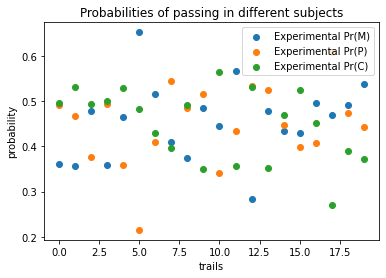
\includegraphics[width=\columnwidth]{figures/plotProb.png}
    \caption{Probabilities of passing in different subjects in different trails}
    \label{fig:plotProb}
\end{figure}
\begin{figure}[h]
    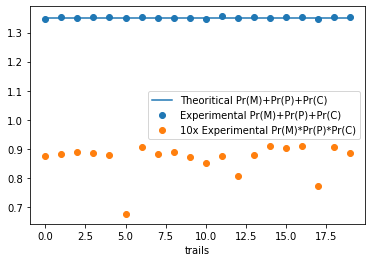
\includegraphics[width=\columnwidth]{figures/plotSumAndProduct.png}
    \caption{Sums and Products of probabilities in different trails}
    \label{fig:plotSumAndProduct}
\end{figure}
\end{document}    